\begin{frame}

\Large Multimodal learning combines different types of data or sensory channels
\end{frame}


\begin{frame}{Introduction}
    \begin{itemize}

    \item We use five senses to perceive
    \item Mimic human learning processes
    \item Combine text, video/images, audio to better understand
    \end{itemize}

\end{frame}

\begin{frame}{Multi-modal Perception}
    \begin{itemize}
        \item A thought on good coffee
        \item Visualize the scene
        \item Sequence of related words and context
        \item Describe them using speech
        \item Exhibit emotions - nostalgic
        \item Some draw the south Indian coffee on a traditional vessels
        \item \(\cdots\)
   \end{itemize}
\end{frame}

\begin{frame}{NLP}
\begin{itemize}
    \item 	[] Word Embedding
    \begin{itemize}
        \item Form dense vectors for every word to capture its semantic nature
        \item Allows similar words to be close in a feature space
        \item Algorithms - HALS, COALS, Word2Vec, GloVe, FastText
    \end{itemize}
\end{itemize}
\end{frame}

\begin{frame}{Word2Vec Model}
\begin{figure}
	\centering
	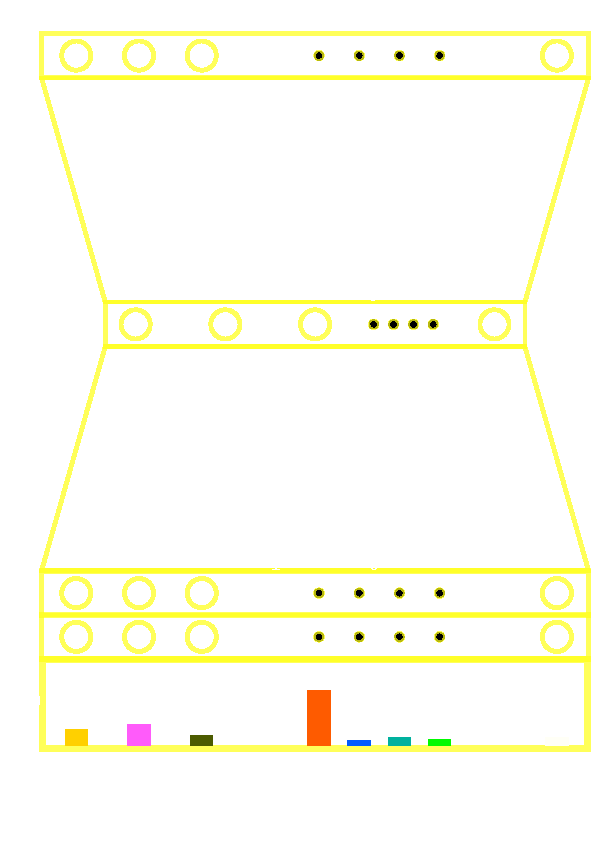
\includegraphics[width=0.35\linewidth]{SoftmaxH1}
\end{figure}
\end{frame}

\begin{frame}{Similar Words for Virus}
    \centering
    \begin{tabular}{|c|c|}
        \hline
        \textbf{Vocab size}& \textbf{Words in the corpus}\\
        \hline
        637722
        & 222502540\\
        \hline
        \hline
        	\hline
        	\textbf{Word}&\textbf{Similarity}\\
        	\hline
        virus,&0.889620\\
        viral&0.785719\\
        (herpesvirus)&0.764385\\
        avirus&0.759567\\
        fluav)&0.757418\\
        polio-virus&0.724740\\
        $\vdots$&\vdots\\
        (vsv;&0.723436\\
        (denv-2)&0.722825\\
        (cowpox)&0.717185  \\
        $\vdots$&\vdots\\
        	\hline
    \end{tabular}
\end{frame}


\begin{frame}{Understanding Long Context}
    \begin{itemize}
        \item Encoder-Decoder Architectures
        \begin{itemize}
            \item Solve the challenge of mapping long input sequences of different lengths
        \end{itemize}
        \item Attention Mechanism: Enables models to focus on relevant information
        \item Transformer Architecture Advantages
        \begin{itemize}
            \item Self attention mechanism
            \item Perform parallel operations
            \item Pretrained and fine-tuning capabilities for a specific content
            \item Deep Network Capabilities
        \end{itemize}
    \end{itemize}
\end{frame}

\begin{frame}{Challenges}
    \begin{itemize}
        \item Deep learning models operate on numeric data
        \item Challenges in converting unstructured inputs to numeric formats
        \item How to combine multi-modal information
        \item Identifying relationship across the senses - both contextual (in text) and spatial (in images)
        \item[] \keywordclr{Connecting thoughts, words and images}
        \item Thought of a dog $\rightarrow$ description in text $\rightarrow$ understand the text $\rightarrow$ translate the meaning into visual representation
    \end{itemize}
\end{frame}

\begin{frame}{Examples of Multi-modal Learning Tasks}
    \begin{multicols}{2}
        \headclr{Text-to-Image Generation}
        \begin{itemize}
            \item \keywordclr{Input} - Chippiparai
            \item \keywordclr{Output} - The Chippiparai is a breed of sighthound from the State of Tamil Nadu in southern India.

            The Chippiparai has typical streamlined sighthound features with long legs and a lean and lithe frame built for speed. The breed is usually white in color, although other colors can be found.
        \end{itemize}
        \vfill\null\columnbreak
        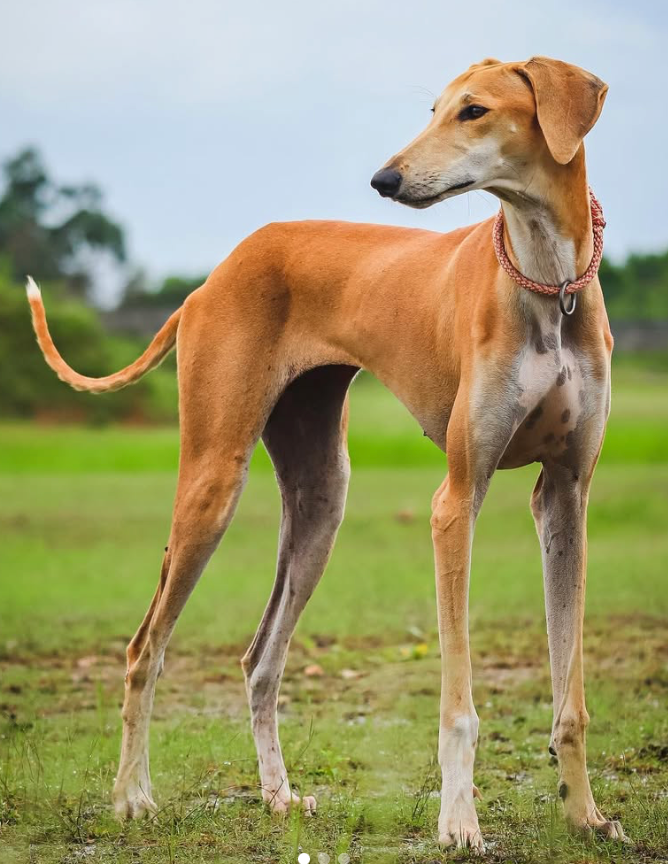
\includegraphics[width=0.7\linewidth]{Images/Chippiparai}

    \end{multicols}
\end{frame}

\begin{frame}{Video based text analysis}
    \begin{itemize}
        \item [] \keywordclr{Input} -  A lecture video (video and audio)
        \item [] \keywordclr{Output}
        \begin{itemize}
            \item classification of the topic
            \item Summary of the lecture, a chapter/section of the topic
            \item Translation to another language,
            \item Create transcription in another language
            \item Identification of words for lip synchronization
            \item $\cdots$
    \end{itemize}
\end{itemize}
\end{frame}

\begin{frame}{Advances in Architecture}
	\begin{itemize}

		\item Transformers - CLIP, DALL-E for combining modalities
		\item Idenify embeddings across modalities
		\item Fusing modalities
		\item Combining contextual and spatial relationships -Develop embeddings that capture deeper relationships
		\item Scalable Systems - Transformers reached its full potential -What next?
		Develop embeddings that capture deeper relationships.
        \end{itemize}
\end{frame}

\begin{frame}{Common patterns}
	\begin{itemize}
		\item Classification
	 	\item Regression
		\item Clustering
	      	\item Dimensionality reduction
	     	\item Contextual Association
	\end{itemize}
\end{frame}


\begin{frame}{State of the art - NLP}
content...
\end{frame}
\begin{frame}{CNN: Convolutional Neural Network}
	\begin{itemize}
		\item CNN: A class of deep learning models designed for image and spatial data
		\item ResNet: Introduces residual connections to improve training of very deep networks
	\end{itemize}
\end{frame}

\begin{frame}{CNN}
	\headclr{Good at extracting the spatial features from data}
	\begin{itemize}
																		           	\item Convolutional Layers: Extract features.
																				\item Pooling Layers: Reduce spatial dimensions.

																				\item Fully Connected Layers: Map features to output.
																				\end{itemize}

\end{frame}

	\begin{frame}{ResNet}
\end{frame}


\begin{frame}{State of the art - Computer Vision}
	advances in CV

\end{frame}


